\chapter{Арга зүй ба системийн зохиомж}

\section{Системийн архитектур (System Architecture)}
Системийн ерөнхий архитектурыг уламжлалт 3 давхаргат (3-Layer Architecture) бүтцээр зохиомжилсон бөгөөд энэ нь өгөгдлийн, логик болон хэрэглэгчийн харилцах цонхны хэсгүүдийг бие даан хөгжүүлэх, турших боломжийг олгосон.

\begin{itemize}
    \item \textbf{Өгөгдлийн давхарга (Data Layer)}: Room Persistence Library ашиглан локал SQLite баазад зурвас, харилцан яриа болон ангиллын мэдээллийг хадгална.
    \item \textbf{Бизнес логикийн давхарга (Domain Layer)}: Тогтмол илэрхийллийн шүүлтүүрийн хөдөлгүүр болон хавтаслах системийн цөм логик байрлана. Энэ хэсэг нь ирж буй зурвасыг таньж, зохих хавтаст оноох үүргийг гүйцэтгэнэ.
    \item \textbf{Танилцуулга давхарга (Presentation Layer)}: XML View систем болон Jetpack Compose ашиглан хэрэглэгчийн хэрэглэгчийн харилцах цонхыг бүрдүүлнэ. ViewModel болон StateFlow ашиглан өгөгдлийн урсгалыг удирдана.
\end{itemize}

\begin{figure}[H]
    \centering
    
\includegraphics[width=0.55\textwidth]{Diagrams/architecture}
    \caption{Системийн ерөнхий бүтэц (Architecture Diagram)}
    \label{fig:architecture}
\end{figure}

Системийн үндсэн бүрэлдэхүүн хэсгүүд нь UI, бизнес логик, өгөгдлийн сан гэсэн 3 давхаргат бүтэцтэй бөгөөд мессежийн өгөгдөл нь Android-ийн богино мессежийн үйлчилгээний сангаас орж ирж, дүрмийн хөдөлгүүрээр шүүгдэн Room өгөгдлийн санд хадгалагдана. UI нь ViewModel/StateFlow-оор дамжин өөрчлөлтийг бодит хугацаанд тусгана.

\section{Өгөгдлийн сангийн зохиомж (Database Design)}
Өгөгдлийн сангийн гол бүтэц, хүснэгт хоорондын холбоосыг ER диаграммаар Зураг \ref{fig:erd} дээр үзүүлэв.

\begin{figure}[H]
    \centering
    
\includegraphics[width=0.55\textwidth]{Diagrams/erd}
    \caption{Өгөгдлийн сангийн ерөнхий бүтэц (ER Diagram)}
    \label{fig:erd}
\end{figure}

\begin{itemize}
    \item \textbf{Categories}: Ангиллын нэр, өнгө, дүрмийн тохиргоо хадгална.
    \item \textbf{Rules}: Түлхүүр үг болон тогтмол илэрхийллийн дүрэм, ангилалтай холбогдоно.
    \item \textbf{Харилцан яриа}: Харилцан ярианы ерөнхий мэдээлэл, ангиллын холбоос.
    \item \textbf{Messages}: Бодит зурвасын агуулга, илгээгч, огноо, харилцан ярианд хамаарал.
\end{itemize}

\section{Нарийвчилсан зохиомж ба Логик дараалал (Detailed Design)}
Системийн хамгийн чухал процесс болох Зурвас автоматаар ангилах'' логикийг UML Sequence диаграммаар (Зураг \ref{fig:seq_diag}) харуулав.

\begin{figure}[H]
    \centering
    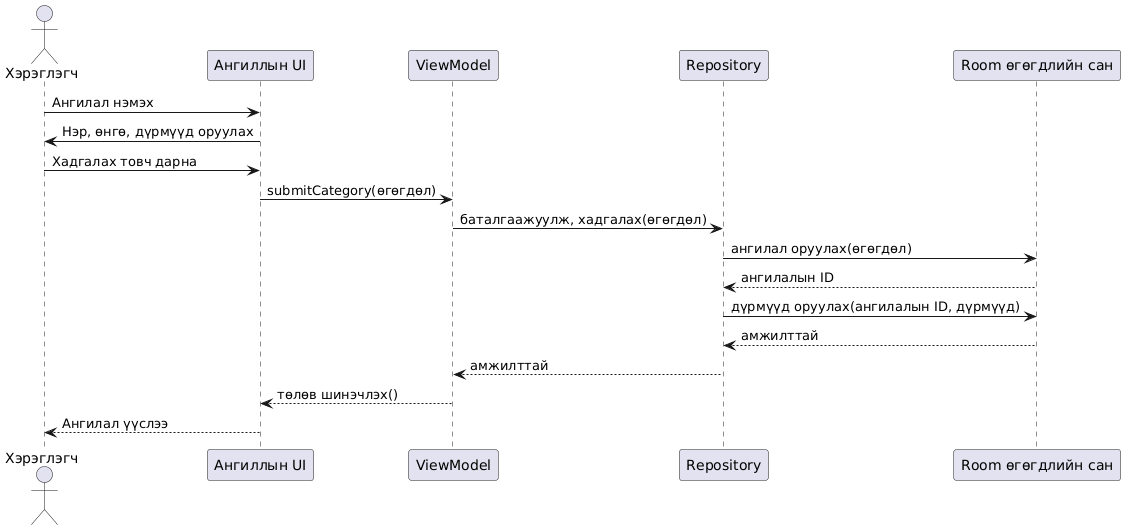
\includegraphics[width=0.85\textwidth]{Diagrams/sequence/category_sequence}
    \caption{Ангилал шинээр үүсгэх (Sequence Diagram)}
    \label{fig:seq_diag}
\end{figure}

Хавтас үүсгэх болон хадгалах логикийг дарааллын диаграммаар (Зураг \ref{fig:seq_category}) харуулав.

\begin{figure}[H]
    \centering
    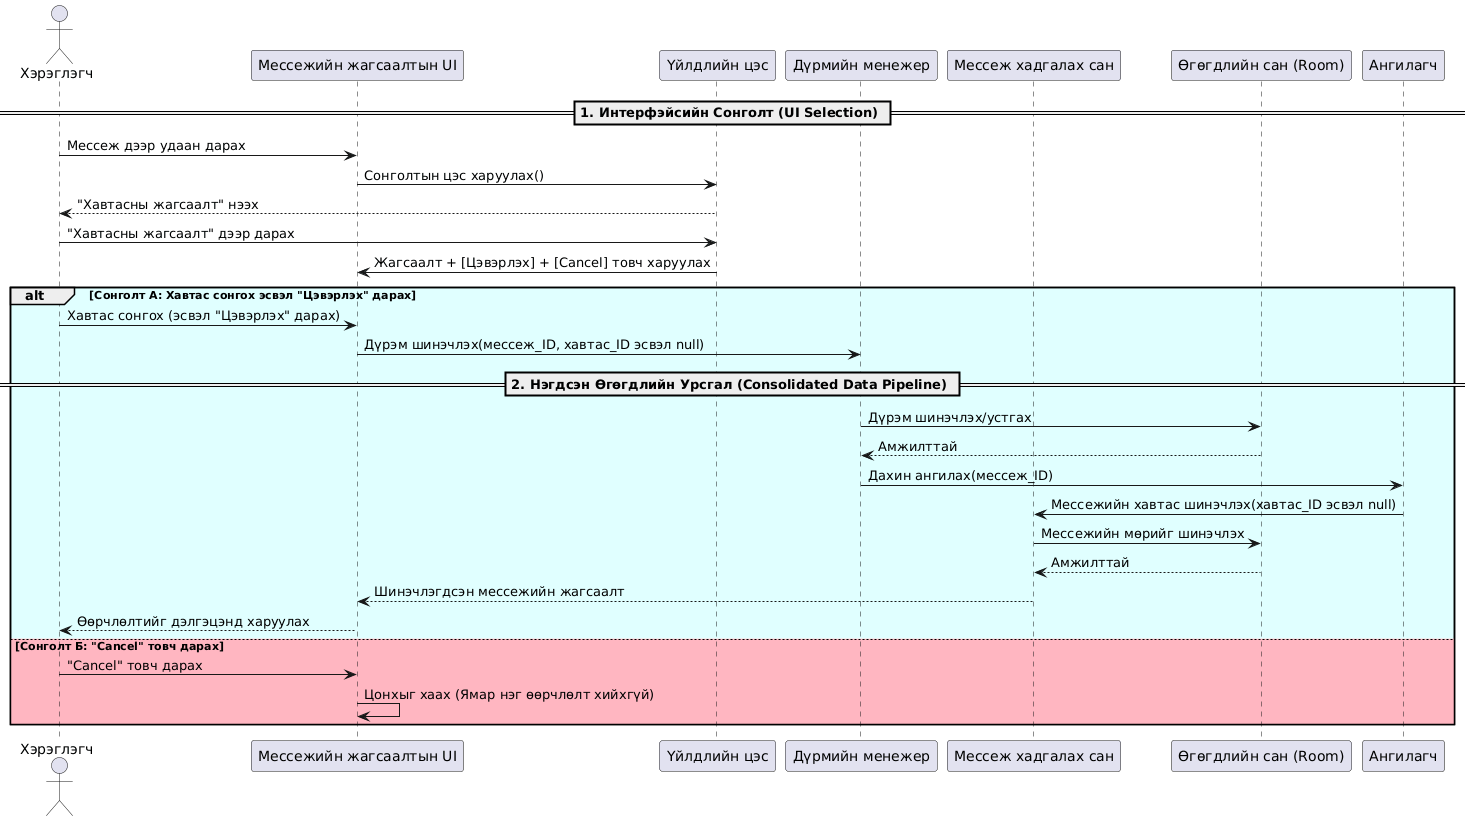
\includegraphics[width=0.85\textwidth]{Diagrams/sequence/assign_folder_sequence.png}
    \caption{Хавтас үүсгэх болон хадгалах дараалал (Sequence Diagram)}
    \label{fig:seq_category}
\end{figure}

Мөн тогтмол илэрхийллийн шүүлтүүрийн ажиллах дотоод дарааллыг Үйл ажиллагааны диаграммаар (Зураг \ref{fig:act_diag}) дүрслэв. Энэхүү логик нь эхлээд энгийн түлхүүр үгийг шалгаж, хэрэв таарахгүй бол илүү нарийн тогтмол илэрхийллийг шалгах замаар системийн гүйцэтгэлийг оновчилдог.

\begin{figure}[H]
    \centering
    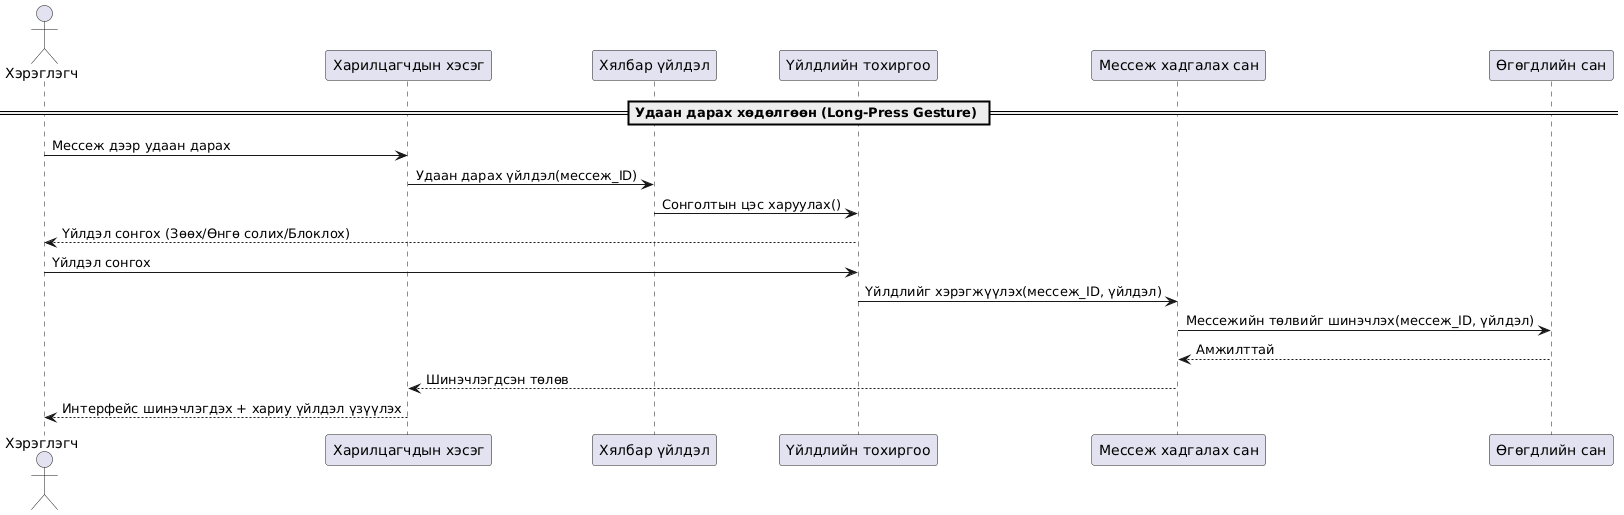
\includegraphics[width=0.85\textwidth]{Diagrams/sequence/long_press_sequence_diagram.png}
    \caption{Удаан дарж гарч ирэх туслах цэсний логик}
    \label{fig:act_diag}
\end{figure}
\subsection{хэрэглэгчийн харилцах цонхны бүтэц ба Үйл ажиллагааны логик} Аппликейшны дэлгэцүүд болон тэдгээрийн хоорондын харилцан хамаарал, удирдлагын логикийг Зураг \ref{fig:class_activity}-д үзүүлэв. Энэхүү хэсэгт нугалдаг төхөөрөмжид зориулсан дасан зохицох хэрэглэгчийн харилцах цонхны зохиомжийг тусгасан бөгөөд нугалдаг утасны удирдлагын зохицуулах арга барилын \cite{foldable_guide} дагууд хэрэгжүүлнэ.
\begin{figure}[H] \centering 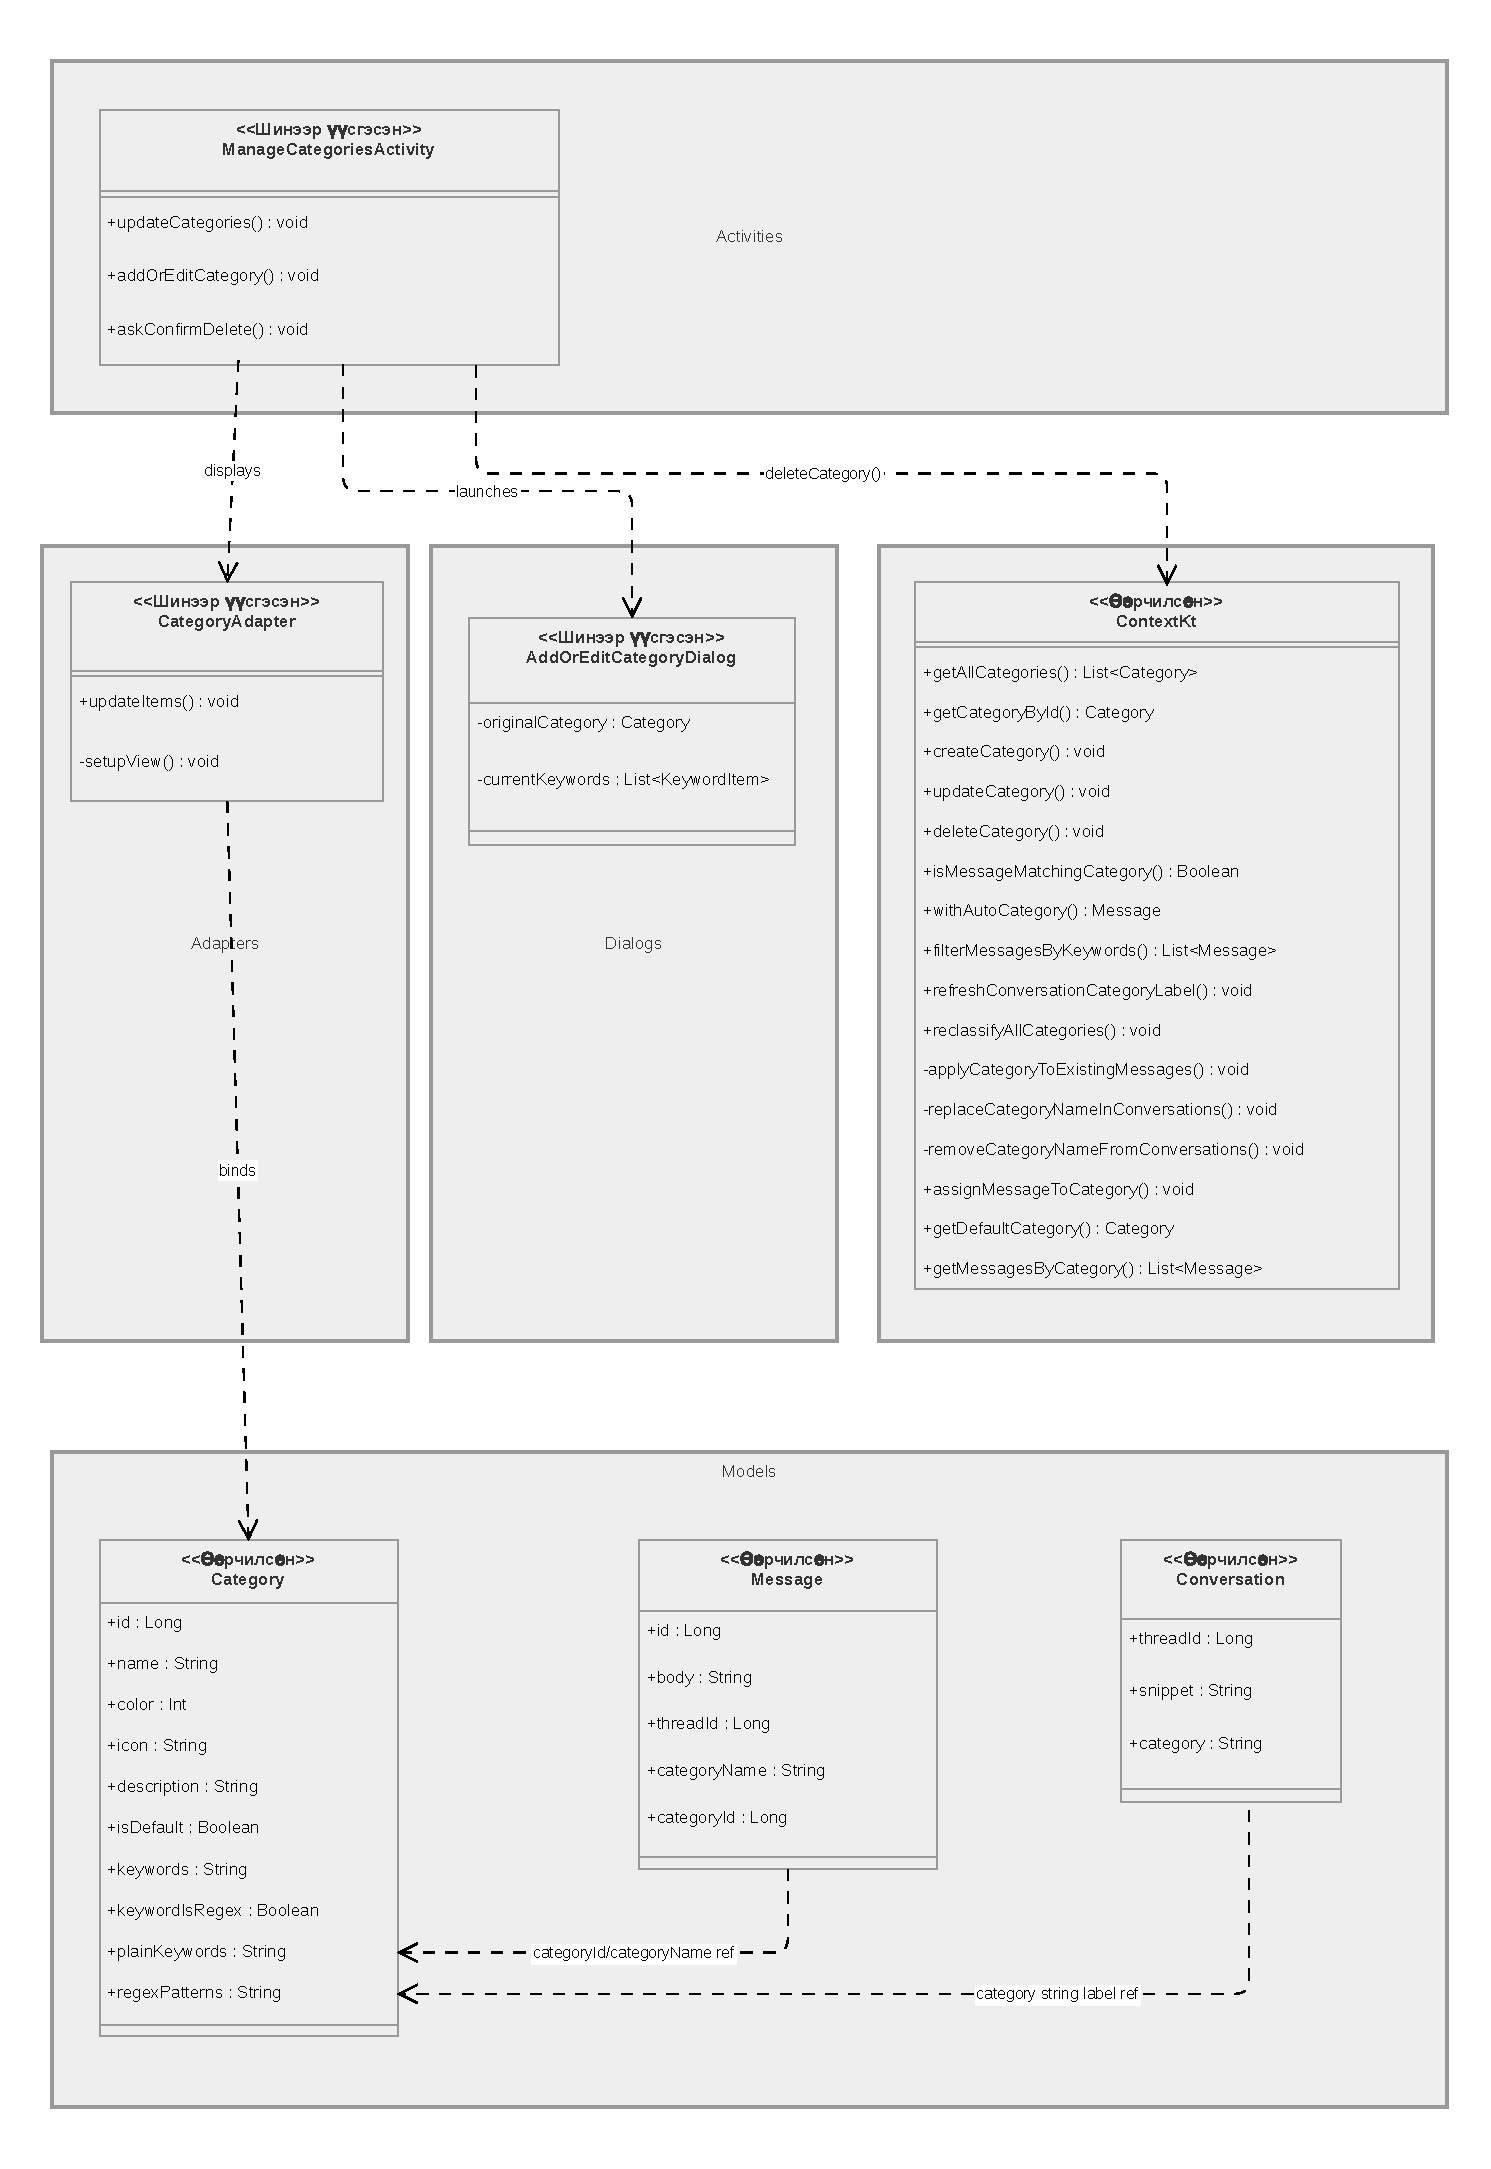
\includegraphics[width=0.85\textwidth]{Diagrams/class/activity.drawio.pdf} \caption{Үндсэн Activity, Fragment болон UI логикийн класс диаграмм} \label{fig:class_activity} \end{figure}
\noindent \textbf{Диаграмд тусгагдсан гол классуудын үүрэг:} \begin{itemize} \item \textbf{NEW Activities}: \begin{itemize} \item \texttt{ManageCategoriesActivity}: Ангиллын жагсаалтыг шинэчлэх (\texttt{updateCategories}), засах цонх дуудах (\texttt{addOrEditCategory}) үйлдлүүдийг удирдана. \item \texttt{ConversationDetailFragment}: Нугалдаг төхөөрөмж дээрх хоёр баганат харагдацыг (\texttt{two-pane}) дэмжих бөгөөд \texttt{threadAdapter}-аар дамжуулан зурвасын урсгалыг харуулна. \end{itemize}
    \item \textbf{Modified Context Logic}: \texttt{ContextKt} класс нь системийн Бизнес логикийн гол цөм бөгөөд дараах өргөтгөл функцүүдийг агуулна:
    \begin{itemize}
        \item \texttt{reclassifyAllCategories()}: Бүх зурвасыг шинээр ангилах.
        \item \texttt{refreshConversationCategoryLabel()}: Харилцан ярианы шошгыг шинэчлэх.
        \item \texttt{filterMessagesByKeywords()}: Түлхүүр үгээр зурвас шүүх.
    \end{itemize}
\subsection{Ангилал болон шүүлтүүрийн системийн бүтэц} Системийн хамгийн чухал хэсэг болох зурвас таних, ангилал үүсгэх болон өгөгдлийн сангийн харилцан хамаарлыг Зураг \ref{fig:class_category}-д үзүүлэв.
\begin{figure}[H] \centering 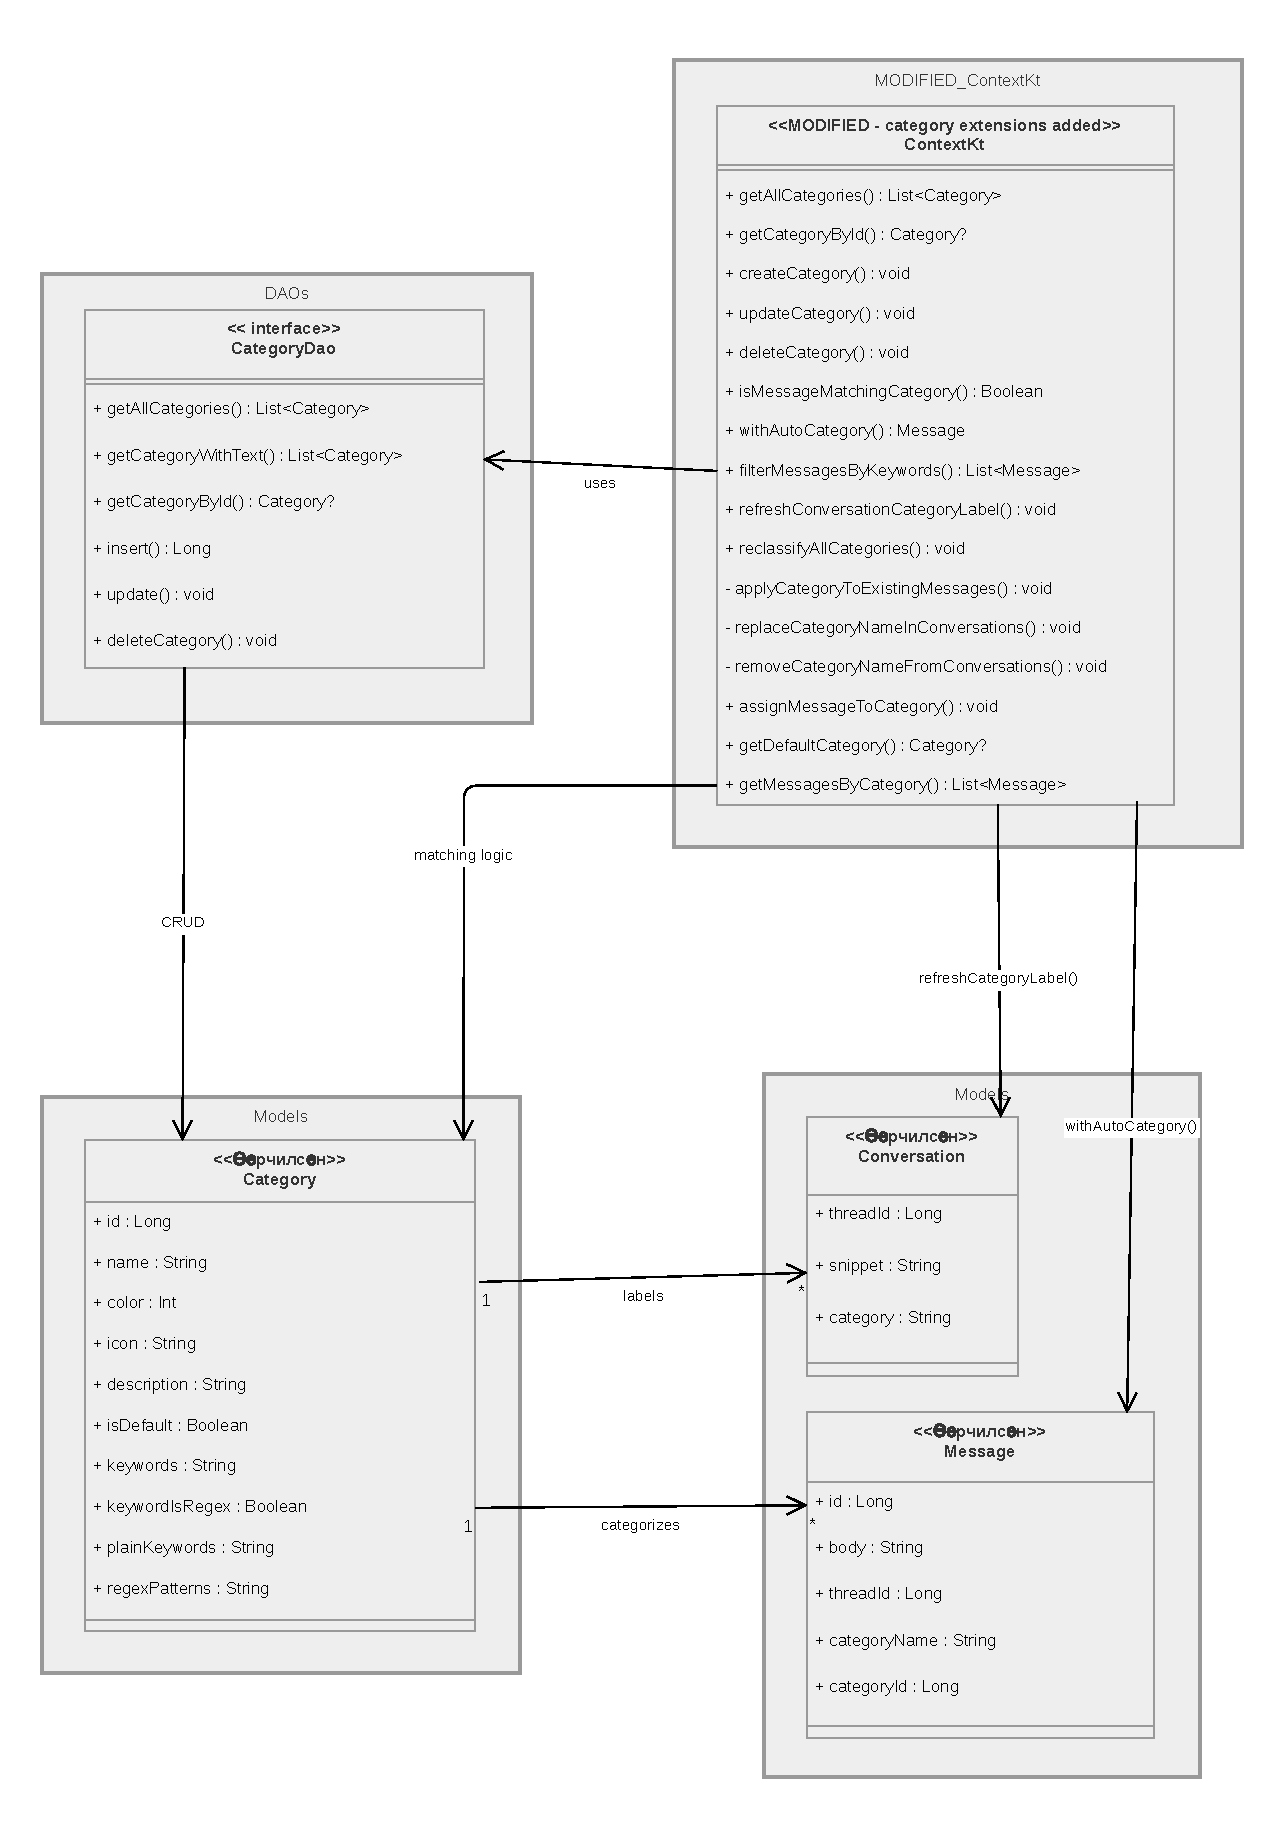
\includegraphics[width=0.85\textwidth]{Diagrams/class/category.drawio.pdf} \caption{Ангилал болон шүүлтүүрийн нарийвчилсан класс диаграмм} \label{fig:class_category} \end{figure}
\noindent \textbf{Бүрэлдэхүүн хэсгүүдийн техникийн тайлбар:} \begin{itemize} \item \textbf{CategoryDao (Шинэ хэрэглэгчийн харилцах цонх)}: Өгөгдлийн сантай харьцах цөм хэрэглэгчийн харилцах цонх бөгөөд ангиллын жагсаалт авах (\texttt{getAllCategories}), түлхүүр үгээр хайх (\texttt{getCategoryWithText}) болон CRUD үйлдлүүдийг гүйцэтгэнэ.
    \item \textbf{Models (Өгөгдлийн загвар)}:
    \begin{itemize}
        \item \texttt{Category}: Шүүлтүүрийн дүрмийг хадгалах модель. \texttt{plainKeywords} болон \texttt{regexPatterns} гэсэн шинэ талбаруудыг ашиглан "Dual-mode" шүүлтүүрийг дэмжинэ.
        \item \texttt{Message}: Ангилагдсан зурвасын мэдээллийг \texttt{categoryId} болон \texttt{categoryName} талбараар дамжуулан \texttt{Category} модельтой холбож өгсөн.
    \end{itemize}
        \subsection{Өгөгдлийн сангийн зохиомж ба Шилжилт} Системийн өгөгдлийн хадгалалт, хүснэгт хоорондын хамаарал болон өгөгдлийн сангийн шинэчлэгдсэн бүтцийг Зураг \ref{fig:db_schema}-д харуулав.
        \begin{figure}[H] \centering 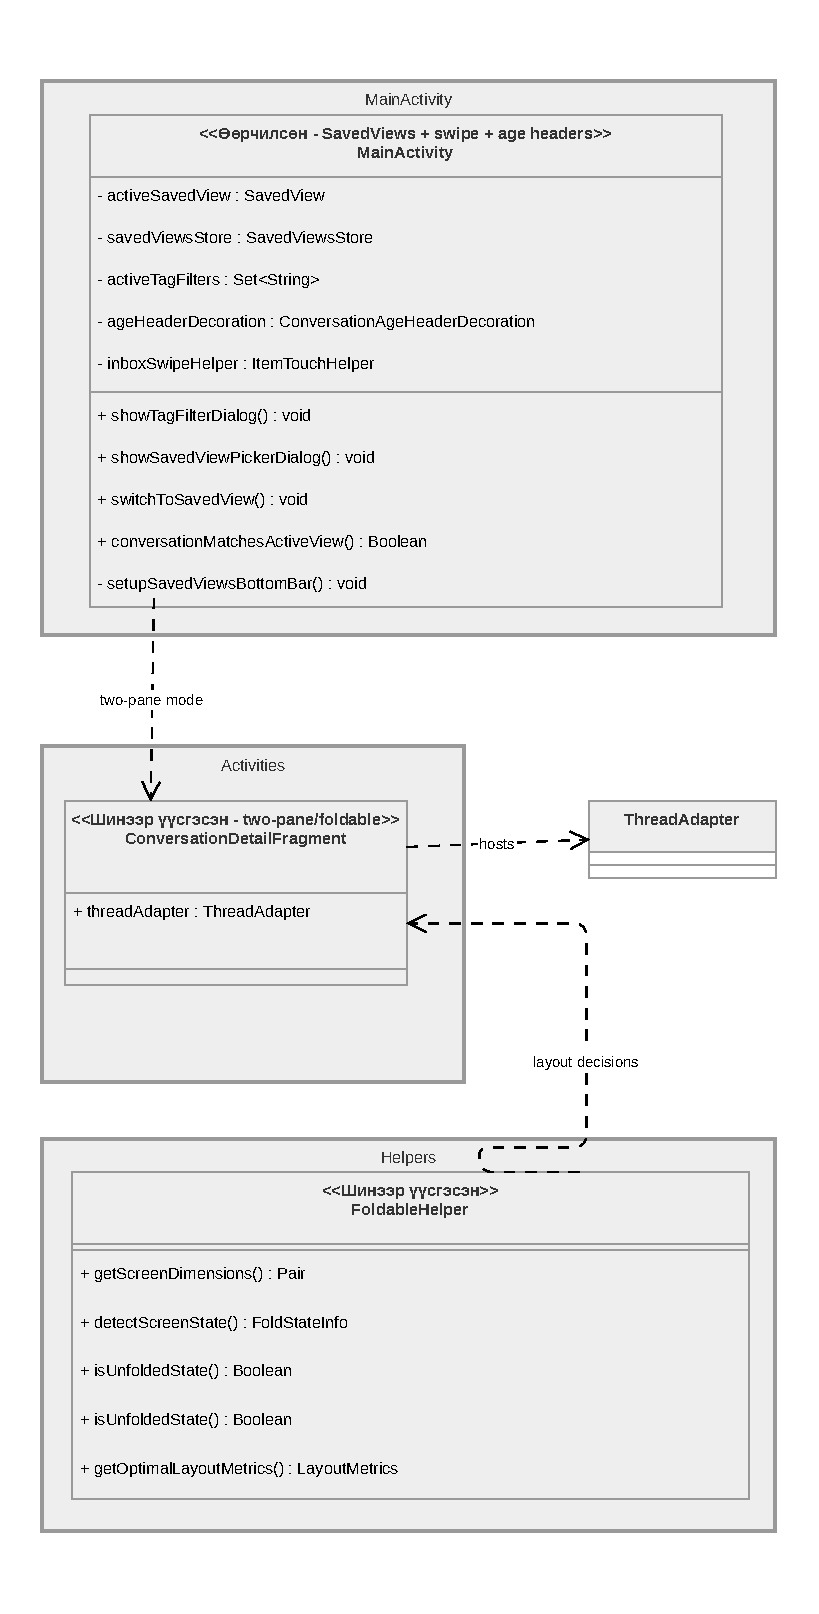
\includegraphics[width=0.9\textwidth]{Diagrams/class/database.drawio.pdf} \caption{Өгөгдлийн сангийн бүтэц болон DAO-ийн класс диаграмм} \label{fig:db_schema} \end{figure}
        \noindent \textbf{Өгөгдлийн сангийн шинэчлэл (Migration Logic):} Төслийн хүрээнд \texttt{MessagesDatabase}-ийн хувилбарыг 10-аас 13 болгон ахиулж, дараах өөрчлөлтүүдийг хийсэн:
        \begin{itemize}
            \item \textbf{MIGRATION 10-11}: \texttt{categories} хүснэгтийг шинээр үүсгэж, \texttt{messages} болон \texttt{conversations} хүснэгтүүдэд ангиллын мэдээллийг хадгалах (\texttt{category}, \texttt{categoryId}) талбаруудыг нэмсэн.
            \item \textbf{MIGRATION 11-12}: Түлхүүр үг нь тогтмол илэрхийлэл (Regex) эсэхийг тодорхойлох \texttt{keywords\_is\_regex} баганыг нэмж, шүүлтийн логикийг өргөтгөсөн.
            \item \textbf{MIGRATION 12--13}: Шүүлтүүрийн логикийг илүү нарийвчлалтай болгох зорилгоор \texttt{categories} хүснэгтэд \texttt{plain\_keywords} болон \texttt{regex\_patterns} багануудыг шинээр нэмж, "Dual-mode" шүүлтийг зэрэг ажиллуулах нөхцөлийг бүрдүүлсэн.
        \end{itemize}
        \noindent \textbf{Гол бүрэлдэхүүн хэсгүүд:} \begin{itemize} \item \textbf{CategoryDao}: Ангиллын мэдээлэлд CRUD үйлдлүүд хийх гол хэрэглэгчийн харилцах цонх. Энд \texttt{getCategoryWithText()}, \texttt{getCategoryById()} зэрэг хайлтын функцүүд шинээр нэмэгдсэн. \item \textbf{Modified Models}: \begin{itemize} \item \texttt{Message}: Зурвас бүр өөртөө \texttt{categoryName} болон \texttt{categoryId} хадгалах болсноор хайлт болон шүүлтийн гүйцэтгэлийг хурдасгасан. \item \texttt{Conversation}: Харилцан ярианы түвшинд ангиллын шошгыг (\texttt{category}) хадгалдаг болж өөрчилсөн. \end{itemize} \end{itemize}
        \item \textbf{ContextKt (Логик өргөтгөлүүд)}: \texttt{Context} класс дээр суурилсан дараах өргөтгөл функцүүд нь системийн ажиллагааг хангана:
        \begin{itemize}
            \item \texttt{isMessageMatchingCategory()}: Зурвасын агуулга тухайн ангиллын Regex эсвэл түлхүүр үгтэй таарч байгааг шалгах логик.
            \item \texttt{withAutoCategory()}: Ирж буй зурвасыг автоматаар ангилж, \texttt{Message} объектыг шинэчлэх.
            \item \texttt{assignMessageToCategory()}: Тодорхой нэг зурвасыг гараар ангилалд оноох.
        \end{itemize}
    \item \textbf{Models \& Config}:
    \begin{itemize}
        \item \texttt{SavedView}: Хадгалсан харагдацын тохиргоог (\texttt{isEditable}, \texttt{position}) хадгална.
        \item \texttt{SavedViewConfig}: Фолдер доторх шүүлтийн нөхцөлүүдийг (\texttt{unreadOnly}, \texttt{matchAllTags}, \texttt{showArchived}) тодорхойлно.
    \end{itemize}
\section{Хэрэглэгчийн харилцах цонхны зохиомж (UI/UX Design)}
Хэрэглэгчийн харилцах цонхыг Material Design 3 стандартын \cite{material_design} дагуу зохиомжилсон.
\begin{itemize}
    \item \textbf{Adaptive Layout}: Нугалдаг төхөөрөмж нээгдэх үед WindowInfoTracker'' ашиглан дэлгэцийн талбайг мэдэрч, хоёр баганат харагдац руу автоматаар шилжинэ.
    \item \textbf{Хадгалсан харагдац}: Хавтас тус бүрт өөрийн гэсэн өнгө оноож, харилцан ярианы жагсаалтыг (Inbox) тухайн өнгөөр зөөлөн будаж (tinting) харуулна.
    \item \textbf{Keyword Manager}: Тогтмол илэрхийлэл болон түлхүүр үгсийг нэг дороос удирдах боломжтой интерактив цонхыг Jetpack Compose-оор хэрэгжүүлсэн.
\end{itemize}
        \item \textbf{ConversationDetailFragment (Шинэ)}: Нугалдаг төхөөрөмж дэлгэгдсэн үед (\texttt{unfolded}) идэвхжих хоёр баганат (\texttt{two-pane}) харагдацын баруун талын хэсгийг хариуцна. Энэхүү fragment нь \texttt{ThreadAdapter}-ийг агуулж, сонгогдсон харилцан ярианы зурвасуудыг харуулна.

        \item \textbf{MainActivity (Өөрчилсөн)}: Програмын үндсэн дэлгэц бөгөөд дараах шинэ боломжуудыг нэгтгэсэн:
        \begin{itemize}
            \item \texttt{SavedViewsStore}: Хадгалсан харагдацуудыг (Folder) удирдах логик.
            \item \texttt{AgeHeaderDecoration}: Зурвасуудыг хугацааны интервалаар бүлэглэх логик.
            \item \texttt{inboxSwipeHelper}: Хэрэглэгчийн тохируулсан шудрах (swipe) үйлдлүүдийг гүйцэтгэх удирдлага.
            \item \texttt{switchToSavedView()}: Шүүлтүүрийн дагуу өөр хавтас руу шилжих үйлдэл.
        \end{itemize}
        \subsection{Түлхүүр үгсийн удирдлагын систем ба Compose зохиомж} Ангиллын дүрмүүдийг (Түлхүүр үг болон Regex) удирдах хэрэглэгчийн харилцах цонхны бүтэц, түүнийг Jetpack Compose-оор хэрэгжүүлсэн зохиомжийг Зураг \ref{fig:class_ui}-д үзүүлэв.
        \begin{figure}[H] \centering 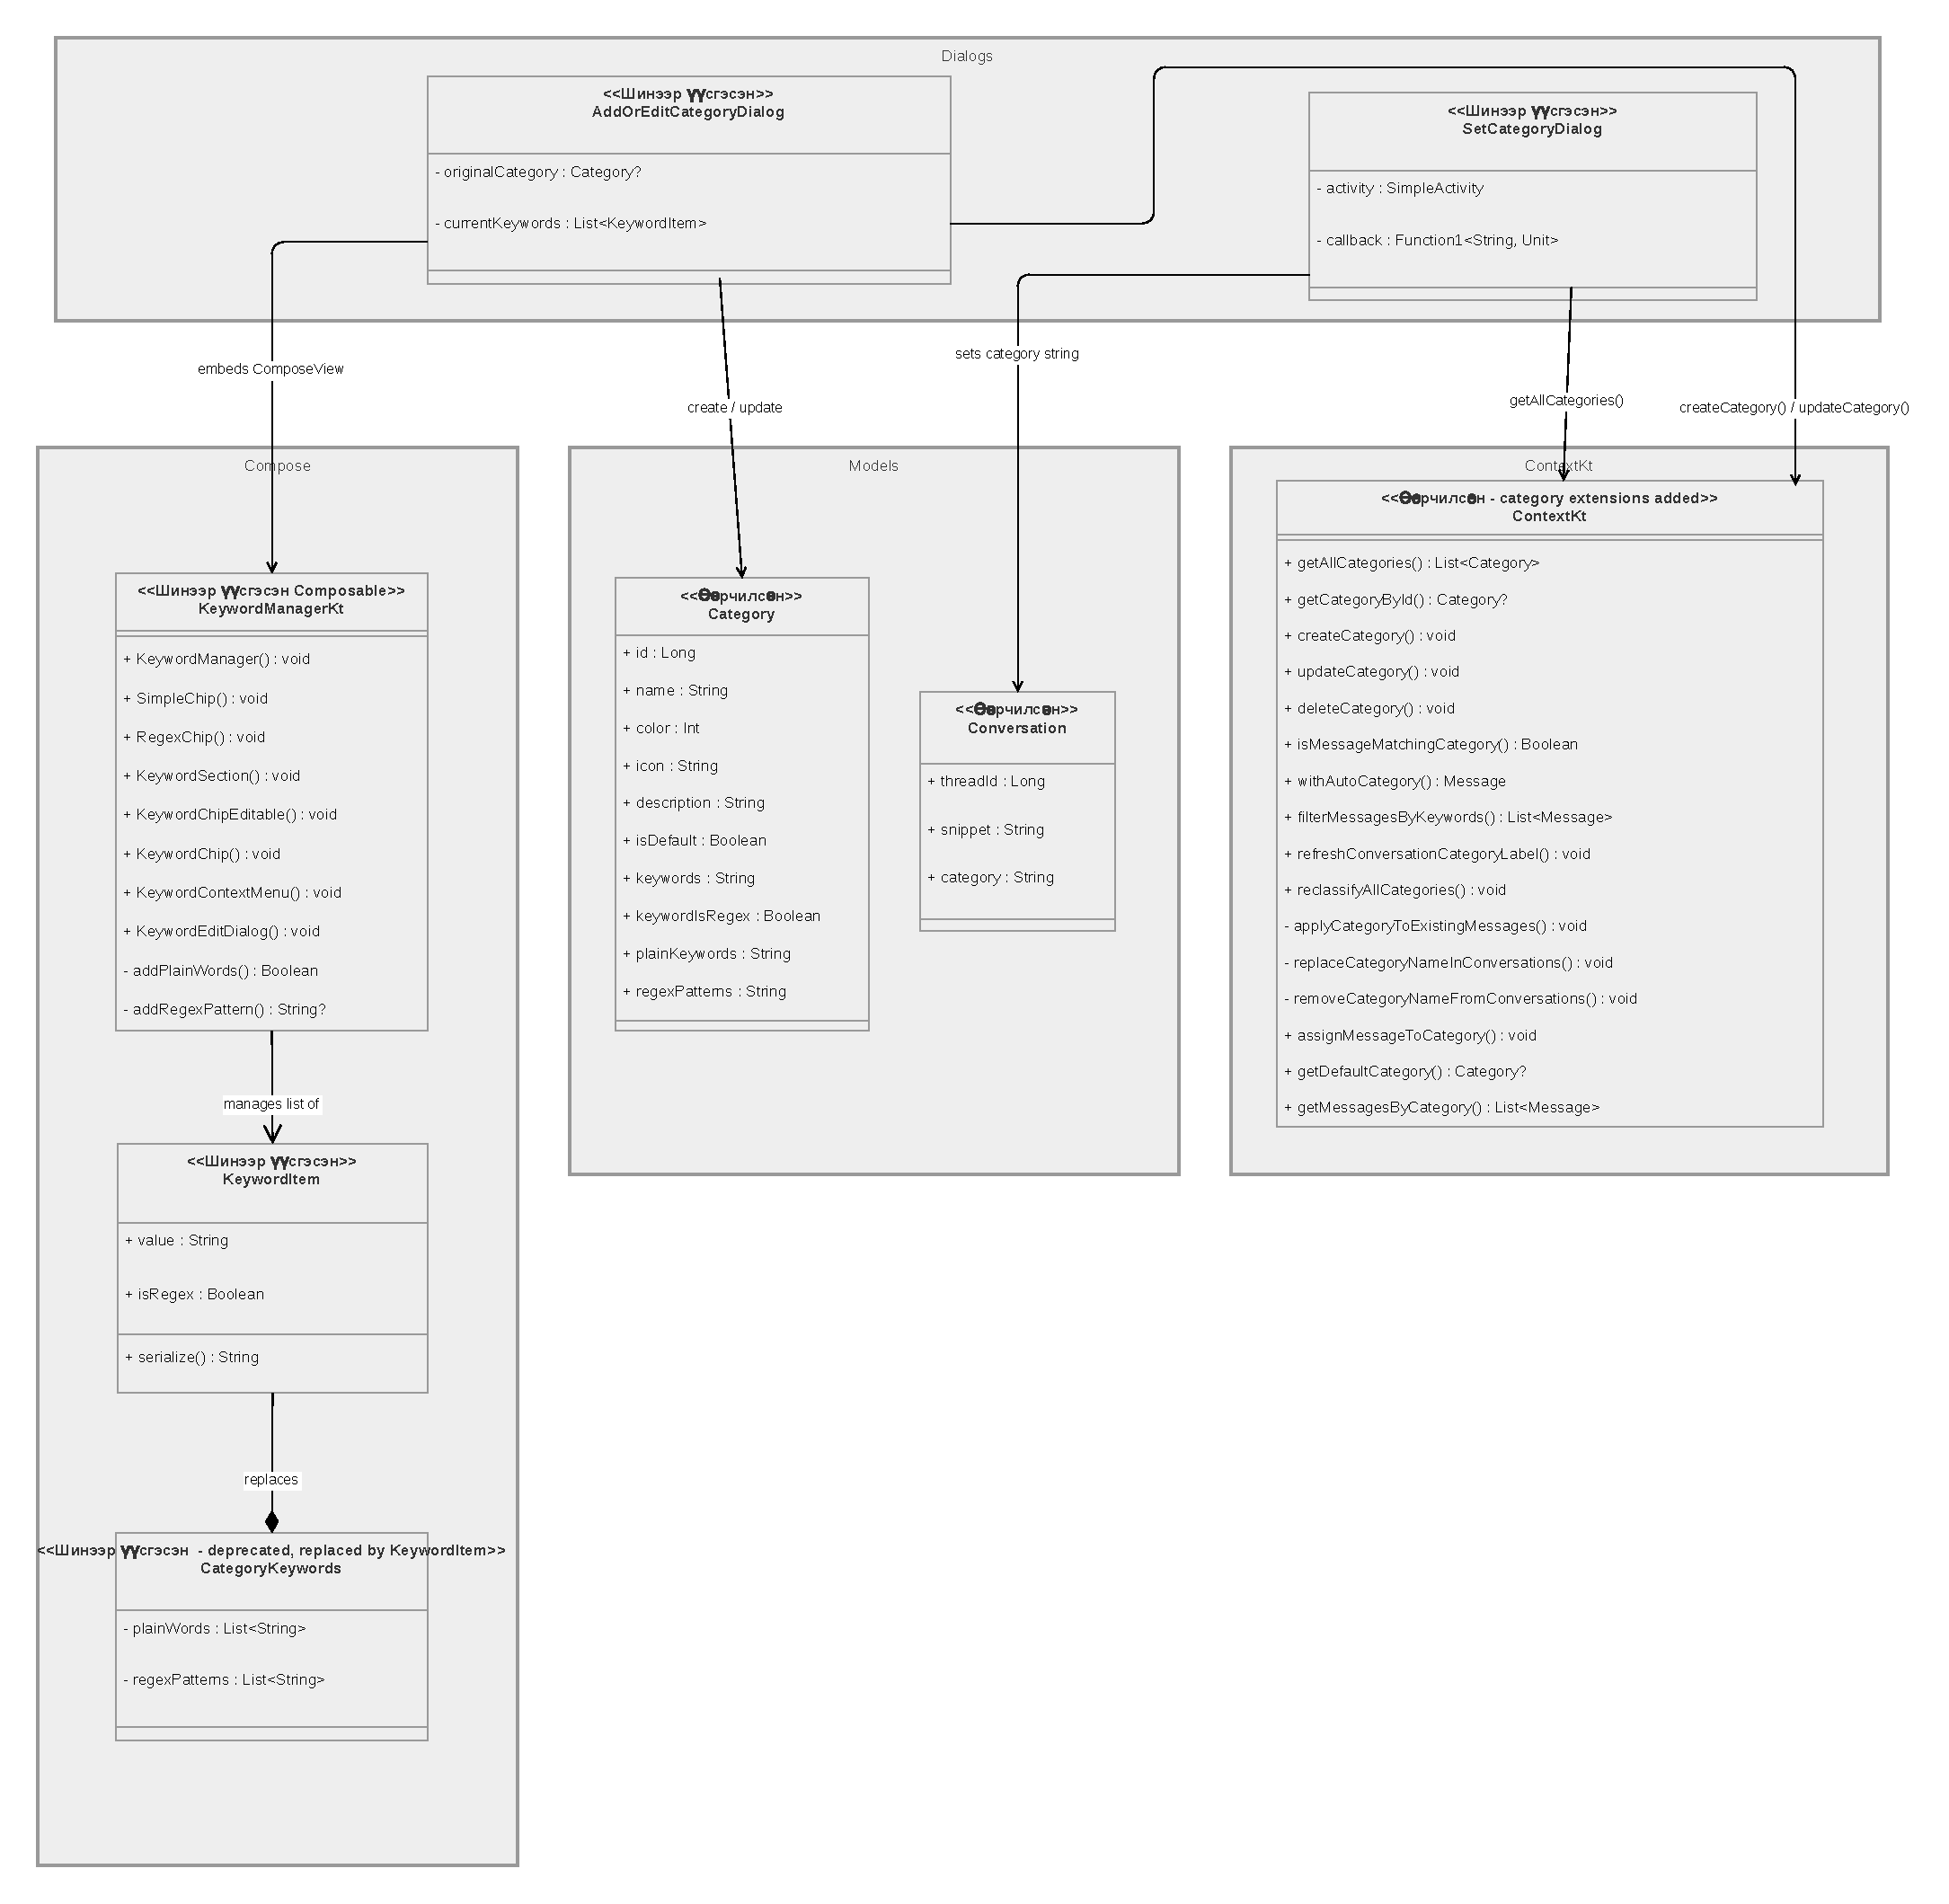
\includegraphics[width=0.85\textwidth]{Diagrams/class/keyboard_ui.drawio.pdf} \caption{Түлхүүр үг удирдах хэрэглэгчийн харилцах цонх болон Compose компонентуудын класс диаграмм} \label{fig:class_ui} \end{figure}
        \noindent \textbf{Диаграмд тусгагдсан гол онцлогууд:} \begin{itemize} \item \textbf{Keyword UI (Compose)}: Түлхүүр үгсийн жагсаалтыг удирдах хэсгийг орчин үеийн Jetpack Compose технологийг ашиглан хэрэгжүүлсэн. \begin{itemize} \item \texttt{KeywordManagerKt}: Түлхүүр үгсийн удирдлагын үндсэн \texttt{Composable} класс. Дотор нь чип хэлбэртэй харагдацууд (\texttt{SimpleChip}, \texttt{RegexChip}), засах цонх (\texttt{KeywordEditDialog}) болон контекст цэс (\texttt{KeywordContextMenu}) зэрэг жижиг компонентуудыг агуулна. \item \texttt{KeywordItem (Шинэ)}: Өгөгдлийг хадгалах болон сериалчлах (\texttt{serialize()}) үүрэгтэй класс. Өмнөх \texttt{CategoryKeywords} классыг орлож, илүү уян хатан байдлыг бий болгосон. \end{itemize}
            \item \textbf{Dialogs (Хэрэглэгчийн харилцах цонх хоорондын холбоос)}:
            \begin{itemize}
                \item \texttt{AddOrEditCategoryDialog}: Уламжлалт \texttt{View} систем болон \texttt{Compose}-ийг нэгтгэсэн гүүр бөгөөд дотроо \texttt{KeywordManager}-ийг агуулна (\texttt{embeds}). Энэхүү диалог нь \texttt{ContextKt}-ийн \texttt{createCategory()} болон \texttt{updateCategory()} функцүүдийг дуудаж өгөгдлийг хадгална.
                \item \texttt{SetCategoryDialog}: Харилцан ярианд ангиллын шошго оноох үйлдлийг гүйцэтгэнэ.
            \end{itemize}

            \item \textbf{Logic \& Data Management}: \texttt{ContextKt} класс нь \texttt{getAllCategories()} функцээр дамжуулан диалогуудыг өгөгдлөөр хангах ба \texttt{Conversation} модельд ангиллын утгыг оноох (\texttt{sets category string}) логикийг гүйцэтгэж байна.
Доод цэсийг эрхий хурууны идэвхтэй бүсэд байрлуулах нь нэг гараар ашиглах эргономикийг сайжруулж, хэрэглэгчийн хурдан шийдвэр гаргалтыг дэмждэг. Шудрах үйлдлүүдээр архивлах, уншсан төлөв солих, хавтас оноох зэрэг мэдээллийг эрэмбэлэх, цэгцлэх урсгалыг нэг алхамд гүйцэтгэх боломж бүрдүүлсэн.

Мөн шошго болон виртуал хавтасны үзэл баримтлалын дагуу ангиллыг физик байрлал гэж бус, шошго дээр суурилсан тусгай харагдац гэж үзнэ. Ингэснээр нэг харилцан яриаг өөр өөр нөхцөлөөр шүүж харах боломжтой бөгөөд хэрэглэгч өөрийн дүрэмд суурилсан хадгалсан харагдацуудыг хурдан үүсгэн ашиглах боломжтой.

\section{Аюулгүй байдлын зохиомж (Security Design)}
Хэрэглэгчийн хувийн зурвасын нууцлалыг хангах үүднээс дараах арга хэмжээнүүдийг зохиомжид тусгав:
\begin{itemize}
    \item \textbf{On-device Filtering}: Зурвасыг ангилах бүх процесс зөвхөн төхөөрөмж дээр локал байдлаар хийгдэх бөгөөд гадны сервер рүү өгөгдөл дамжуулахгүй.
    \item \textbf{Local-first Database}: Өгөгдлийн сан нь Android-ийн App Sandbox дотор тусгаарлагдсан тул бусад аппликейшн шууд хандах боломжгүй.
\end{itemize}

